\chapter{Нейронне імпульсне радіо}
\label{ch:neuron}

%%%%%%%%%%%%%%%%%%%%%%%%%%%%%%%%%%%%%%%%%%%%%%%%%%%%%%%%%%%%%%%%%%%%%%%%%%%%%%%
\section{Недоліки класичного імпульсного радіо}

Основною сферою застосування надширокосмугової радіоелектроніки сьогодні стає
інтернет речей. Основними чинниками для цього стали високий рівень 
інформаційної безпеки, порівняно низький рівень споживання електроенергії та
стійкість до вузькосмугових завад. В електромагнітних задачах інтернету речей,
робота таких пристроїв на маленькій відстані є, скоріш, перевагою, а ніж 
недоліком - цей чинник зменшує радіо-забруднення приміщення.

В оглядовій роботі \cite{imp:ChannelImplementation} приведені основні схеми
роботи не стробоскопічного імпульсного радіо, що використовуються в 
різноманітних сферах починаючи з телекомунікації і закінчуючи радарними 
задачами, які можна узагальнити наступною схемою (Рис.~\ref{fig:emp_radio}).

\begin{figure}[htbp] \begin{center}
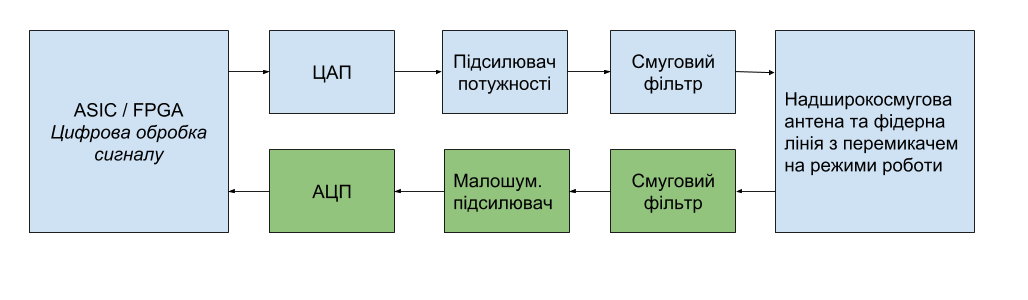
\includegraphics[scale=0.45]{classical_radio}
\caption{Класична схема імпульсного радіо} \label{fig:emp_radio}
\end{center} \end{figure}

Існуючий принцип аналогової обробки прийнятого імпульсного радіосигналу 
успадковані від схемотехніки, що використовувались для гармонійних сигналів 
\cite{imp:ComunicationsOverview}. Тобто, для обробки отриманого з антени 
електричного струму використовується послідовна фільтрація та підсилення з 
подальшим оцифровуванням за допомогою АЦП і цифрової обробки в модулях FPGA 
(Рис.~\ref{fig:emp_radio}).

Кожен з послідовних етапів аналогової обробки, направлений на покращення 
окремої характеристики сигналу неминуче впливає і на інші його характеристики,
що накопичує похибку та губить частину інформації про сигнал:

\begin{enumerate}
	\item фільтрація разом з інформацією про шум частково зачіпає спектр, 
	а відповідно і форму корисного сигналу і не прибирає шум повністю;
	\item кавзі-лінійне підсилювання, також незначним чином впливає на 
	форму імпульсу, за рахунок нелінійності амплітудної і частотної 
	характеристики, а також підсилює не відфільтрований шум;
	\item аналогово-цифрове перетворення сигналу губить частину інформації 
	сигналу та шуму за рахунок дискретизації, що також ускладнює числову 
	обробку
\end{enumerate}

Таким чином на числову обробку потрапляє дещо видозміненій від початкового
сигнал. Також сам алгоритм числової обробки в модулі FPGA, зазвичай,
вибирається простим, через умову обробки сигналу в квазі-реальному часі.

Серед методів обробки сигналу в модулях FPGA, з лінійною складністю по часу 
виконання, можна виділити сімейство методів корелятивного порівняння, що 
базується на фільтрі Калмана. Ці методи, фактично, порівнюють отриманий сигнал 
з еталонним і повертають коефіцієнт кореляції, чого достатньо для бінарної
класифікації наявності сигналу.

В ближній зоні антени, де форма сигналу сильно залежить від напрямку 
спостереження \cite{imp:Wu1985, imp:Sodin1992-10, my:Telecom2018}, що призводить 
до падіння точності роботи описаного підходу порівняння з еталоном. Також, 
погіршання якості роботи кореляційних алгоритмів, впаде при прийманні сильних 
електромагнітних імпульсних хвиль, часова залежність яких теж може значно 
змінюватись.

Імпульсні надширокосмугові радіотехнічні пристрої мають теоретичні переваги 
над вузькосмуговими в плані інформаційної ємності, але через складність 
обробки надширокосмугових сигналів, на практиці, не вдається використовувати 
ці переваги повною мірою \cite{imp:ChannelLimitations}.

%%%%%%%%%%%%%%%%%%%%%%%%%%%%%%%%%%%%%%%%%%%%%%%%%%%%%%%%%%%%%%%%%%%%%%%%%%%%%%%
\section{Імпульсний радіоприймач на базі апаратної нейронної мережі}

Всі задачі випромінювання, розповсюдження чи дифракції хвилі є розв'язком
деяких параметричних рівнянь відносно компонентів струму чи компонентів 
поля. Коли аналітичне розв'язання такого рівняння знайти не вдається, а 
числовий метод розв'язання має значну математичну складність, доцільно 
використати штучні нейронні мережі (ШНМ) прямого поширення та методи їх 
навчання для пошуку розв'язання.

Рівень оптимізації сучасних програмних інструментів машинного навчання, таких 
як CUDA та Tensorflow, а також рівень розвитку апаратних інструментів GPU/ASIC
дозволяють аналізувати часові послідовності простими моделями за час порядку 
мілісекунди, що дозволяє використовувати такі інструменти при роботі з 
сигналом у квазі-реальному часі, опрацьовуючи сигнал після АЦП. Недоліком 
такого методу може стати висока ціна кінцевих виробів. З іншого боку, галузь 
що швидко розвивається - аналогові штучні нейронні мережі, на які можна подати 
сигнал з антени напряму. Такі пристрої широко застосовуються радіотехніками
в галузі когнітивного радіо \cite{imp:Husseini2010}, а також адаптивних 
вузькосмугових антенних систем \cite{imp:Zbynek2002}. В цих задачах, 
апаратні ШНМ мережі використовується для оптимізації деяких параметрів 
прийому-передачі сигналу в режимі реального часу.

Останнім часом технічний розвиток в галузі апаратних штучних нейронних мереж 
дозволив виготовляти аналогові нейронні мережі прямого поширення різного типу,
таких як: FCNN, RNN, LSTM, GRU, HMM, CNN, UNet та інші. Проаналізуємо 
можливість застосування цих технологій для задач класифікації отриманого 
сигналу (sequence-to-label) та визначення його присутності в кожен момент 
часу (sequence-to-sequence). Результат розв'язання таких задач аналізу даних
дозволить оцінити практичну цінність \textcolor{red}{такого методу} обробки 
радіосигналу в різних задачах прикладної електродинаміки: радіолокації, 
телекомунікації, вимірювання, зондування, тощо. 

\begin{figure}[htbp] \begin{center}
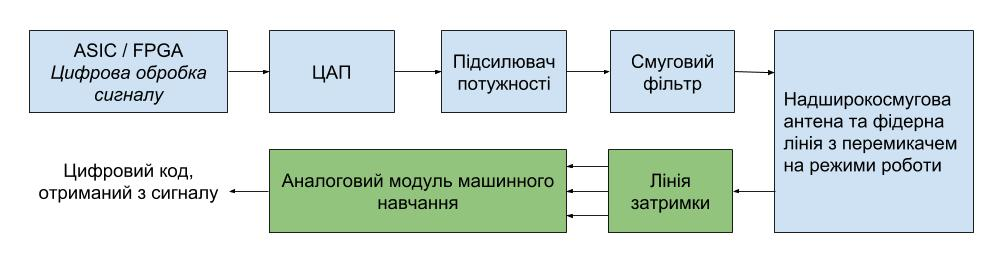
\includegraphics[scale=0.45]{neuron_radio}
\caption{Схема імпульсного радіо на нейронній схемотехніці} 
\label{fig:neural_radio}
\end{center} \end{figure}

Штучна нейронна мережа тут є електричним колом, внутрішня передавальна 
функція якого визначається добутком набору числових матриць. Таким чином 
задача обробки прийнятого радіосигналу зводиться до пошуку необхідних 
матричних параметрів. Для цього гарно підходять градієнтні методи навчання 
з учителем, де конкретна імплементація процесу тренування та набір 
тренувальних даних залежатиме від типу задачі, що розв'язується.

Оптимальною нейронною архітектурою для кіл обробки радіосигналу стане
схема encoder-decoder через свою універсальність \textcolor{red}{[ПОСИЛАННЯ]}. 
В цій архітектурі нейронна мережа топологічно і за значенням розбивається на 
дві частини, перша частина трансформує вхідну часову послідовність в деякий 
набір параметрів, які однозначно характеризують вхідний сигнал. Кажучи 
математичною мовою, encoder проектує вхідний сигнал на деякий ознаковий
простір. Друга частина мережі, decoder, перетворює набір ознак в ту якісну 
або кількісну характеристику, яку передбачає постанова задачі. Наприклад,
для задачі телекомунікації - це інформаційне повідомлення, або для радарної 
задачі - це положення та тип цілі. Такий підхід забезпечить повторне 
використання попередньо-навчених encoder-ів для різноманітних задач 
радіофізики. Апаратна можливість додати декілька різних декодерів в 
електричні кола радіоприймальної схеми зробить цю концепцію промислово 
придатною.

Так як тип вихідного сигналу, що продукує апаратна нейронна мережа залежить
лише від активаційної функції вихідного нейрону, повертати вона може, як 
аналоговий сигнал, так і цифровий. Цифровий сигнал можна отримати ступеневою 
активаційною функцією (персептрон Розенблата) та зручно використовувати 
описаний пристрій, як мереживний інтерфейс комп'ютера, чи джерело керуючого 
сигналу для робототехніки. Аналоговий вихід, в свою чергу, відкриває безліч 
перспектив перед застосуванням надширокосмугового радіо в повністю 
аналогових технічних пристроях, що до цього було неможливо.

Запропонований винахід принципово відрізняється від прототипів методом 
виділення корисної інформації з прийнятого сигналу. В основу існуючих
пристроїв покладено принцип послідовного цифрування та обробки, коли 
запропонована схема не потребує цифрування сигналу для його обробки 
методами машинного навчання. Запропоновано схему можна використовувати як 
при стробоскопічному підході так і при послідовному. Як і класична схема 
імпульсного радіо, запропонована схема передбачає можливість застосовувати 
одну і ту ж антену для передачі та прийму сигналу. Також, використання 
нейропроцесору не виключає застосування традиційних методів аналогової обробки:
підсилення, фільтрація.

Важливим аспектом є те, що використання ПЗУ дозволить програмувати нейронний 
процесор може бути перепрограмований, шляхом встановлення нових
параметрів нейронів, що дає змогу змінювати технічні характеристики 
пристроїв без їх заміни.

Серед переваг нейропроцесорного радіо, що стосуються інтернету речей та 
носимої електроніки - енергоефективність, про що витікає з висновків авторів 
робіт з аналогових нейропроцесорів \cite{imp:AnalogLSTM}.

Також, перспективним напрямком дослідження в області нейронного радіо є 
застосування імпульсних штучних нейронних мереж замість штучної нейронної 
мережі прямого поширення. Тренування таких мереж здійснюється шляхом 
самоорганізації системи під зовнішнім впливом з позитивним підкріпленням. 
Такі мережі простіше виконати у виді аналогової мікросхемотехніки ніж мережі
прямого розповсюдження і їх застосування є більш природнім для задач 
прикладної електродинаміки. З огляду малого обсягу інструментального 
апарату для навчання таких моделей цей підхід в даному досліджені не 
розглядається, але швидкий розвиток подібних технологій залишає їх 
дослідження перспективним в майбутньому.

%%%%%%%%%%%%%%%%%%%%%%%%%%%%%%%%%%%%%%%%%%%%%%%%%%%%%%%%%%%%%%%%%%%%%%%%%%%%%%%
\section{Формування тренувальних даних}

Розглянемо задачу, односторонньої передачі інформації через нейронне радіо. 
В якості передавальної антени розглядається антена типу LIRA. Для спрощення, 
в якості приймальної антени розглянемо ідеальний надширокосуговий вимірювач 
напруженності електричного поля, який не впливає на форму отриманого сигналу,
що нівелює вплив приймальної антени на отриманий сигнал. Сигнал з приймальної 
антени подається на деяку апаратну нейронну мережу. Напруженість електричного 
поля породжене випромінювальною антеною $ \vect{E}_{tx} $ можна знайти в 
довільній точці спостереження при довільному збуджені з урахуваннями ефектів 
ближньої зони користуючись згорткою \eqref{eq:duhamel} по перехідній функції 
$ \vect{E}_0 $. Тоді отриманий радіосигнал з детектора поля буде пропорційний 
до компонентів напруженості електричного поля випромінювальної антени. 
Здійснюючи гіпотетичне вимірювання в такій площині, що спостерігається $ OX $ 
компонента напруженості поля, а приймальна лінія ідеально узгоджена і немає 
втрат, отриманий сигнал матиме вигляд:

\begin{equation}
f_{rx} \left( \vect{r}, t \right) = 
\int_0^t \derivat{f_{tx}}{\tau} \vect{E_0} (\vect{r}, t - \tau) d \tau,
\end{equation}
%
де $ \vect{E_0} $ - перехідна функція передавальної антени типу LIRA, а 
$ f_{tx} (t) $ - форма сигналу, що збуджує передавальну антену

Метою даного моделювання є пошук оптимальної нейронної архітектури, а також 
її вагових коефіцієнтів, що дозволить співвіднести прийнятий сигнал 
 з деяким типом збудження на передавачі в умовах 
завад, та з урахуванням деяких ефектів ближньої зони.

Тренувальний набір даних для цієї задачі складатиметься з пар часових 
послідовностей - струм збудження передавальної антени $ f_{tx} (t) $ та струм, 
що буде отримано приймачем $ f_{rx} (t) $ при різних розташуваннях 
приймача $ \vect{r} $ відносно системи координат передавача, введеної як на 
Рис.~\ref{fig:pdisk}. Для максимально правильного функціонування мережі в 
умовах моделі, набір тренувальних даних повинен містити вичерпну інформацію про 
поведінку поля у всій область функціонування антенної системи, а тобто містити 
вимірювання в ближній і дальній зонах. Користуючись визначенням дальньої зони,
отримуємо максимальне віддалення від джерела, де необхідно проводити 
вимірювання - $ 0 \leq z \leq 8R $. Користуючись направленістю антен типу 
LIRA, обмежимо радіус поперечного зрізу циліндричної області, де проводяться 
вимірювання $ 0 \leq \rho \leq R $, а користуючись симетрією джерела розглянемо 
не весь зріз, а лише його першу чверть $ 0 \leq \varphi \leq \pi / 2 $.

Таким чином просторовий об'єм region of interest складає $ \pi R^2 / 2 $. 
З огляду на низьку сходимість деяких алгоритмів навчання заповнимо 
отриманий region of interest великою кількістю 10000 випадкових рівномірно 
розподілених уявних вимірювань для тренувального набору даних, а також
в чотири рази меншим вілідаційним набором - 2500 семплів. Для наближення 
моделі до реальних умов до кожного з семплів додамо деяку випадкову заваду,
такий підхід відомий в літературі, як задача аналізу AWGN каналу, де енергія 
шуму визначається як квадрат середнього відхилення, що продемонстровано 
на Рис.~\ref{fig:P4AWGN}.

\begin{figure}[htbp] \begin{center}
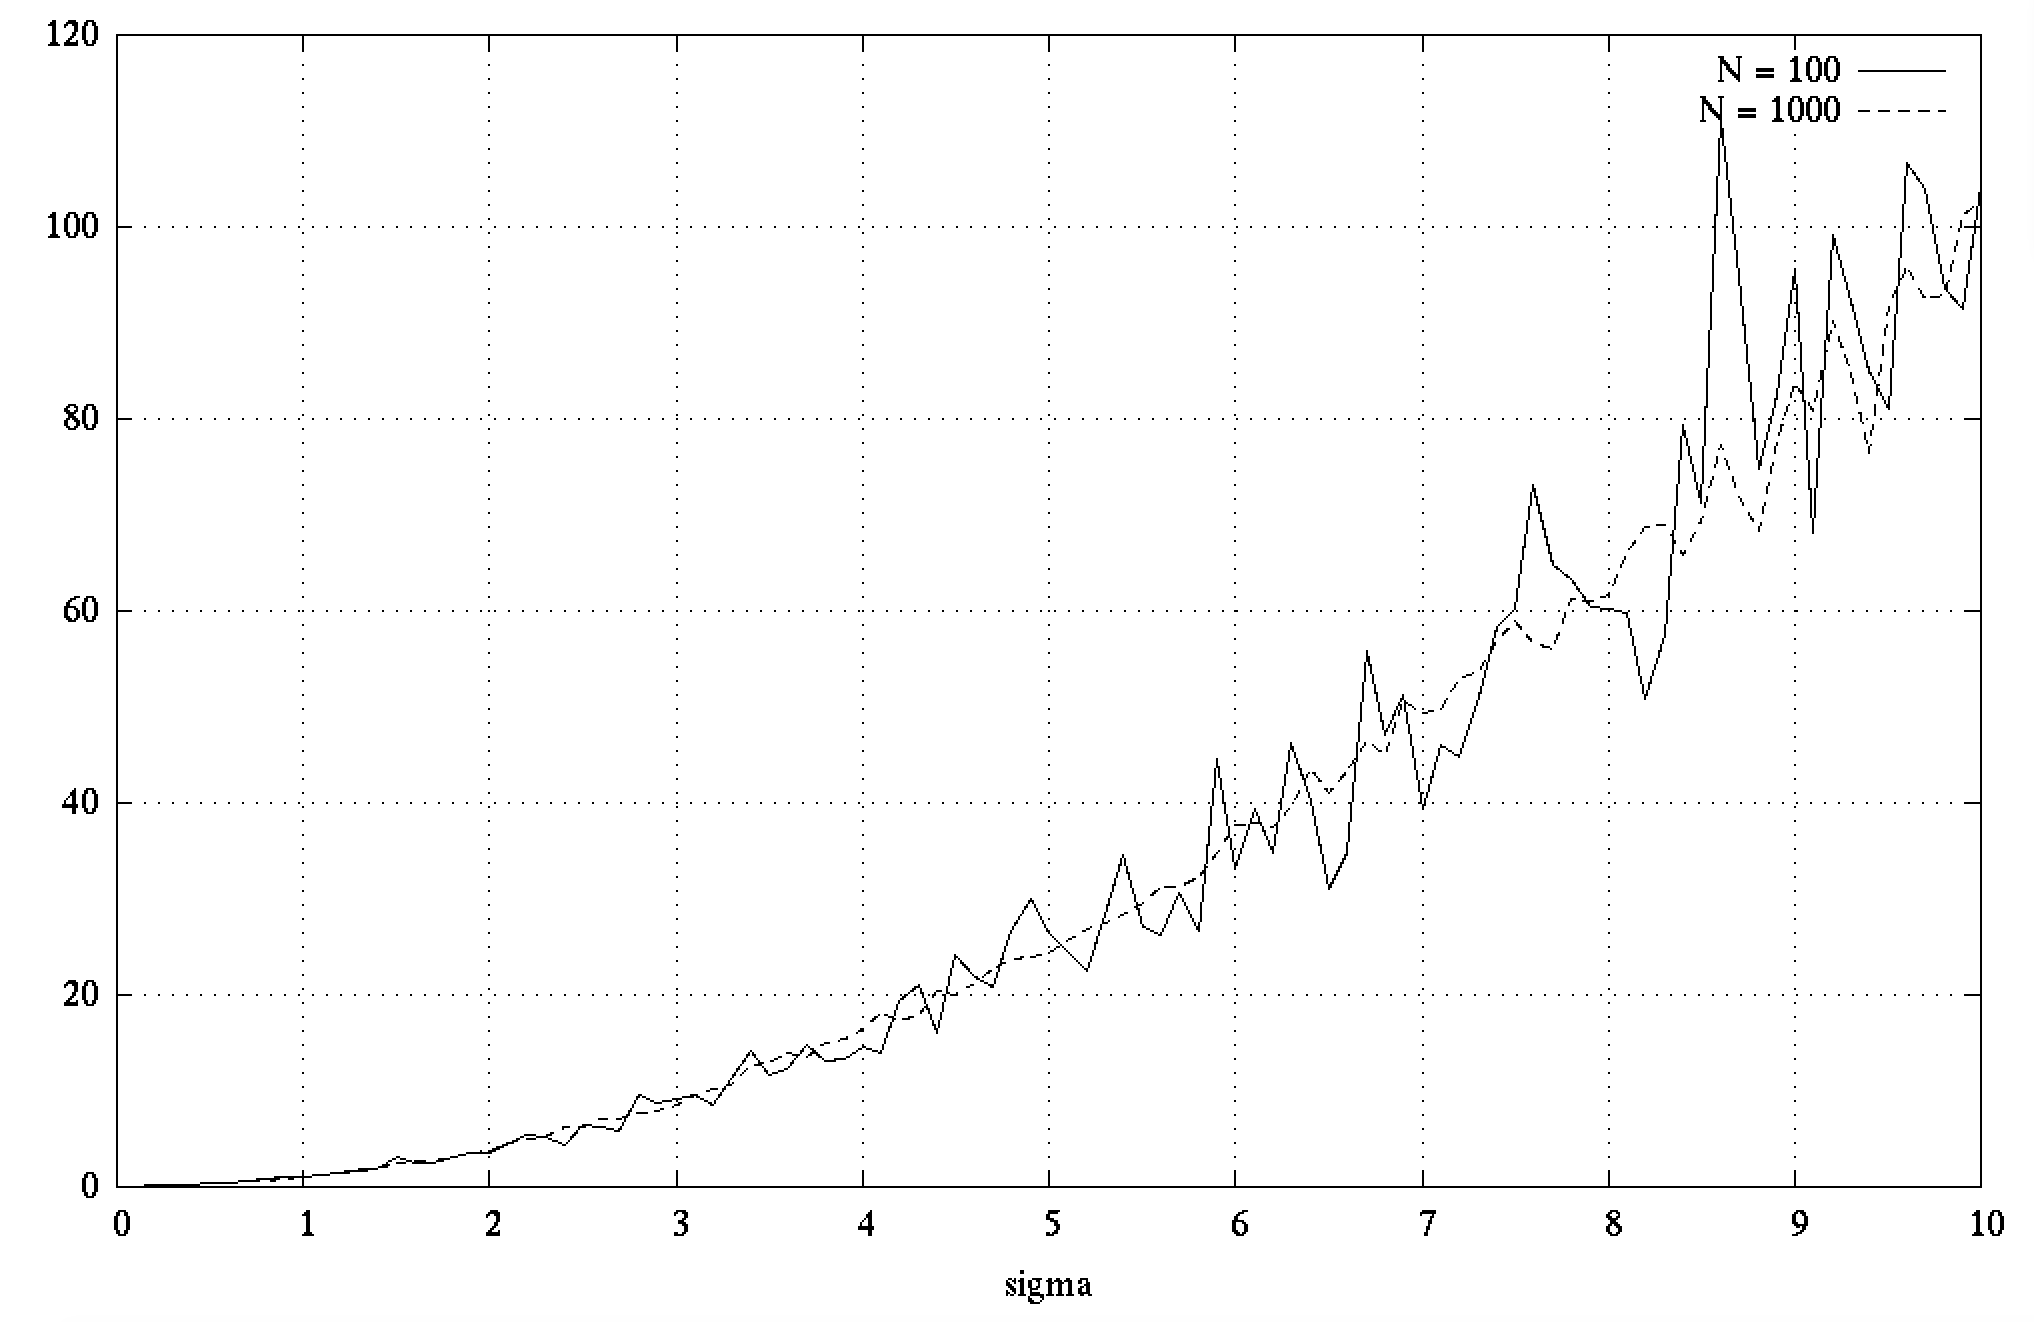
\includegraphics[scale=0.4]{P4AWGN}
\caption{Енергія моделі білого шуму в залежності від параметру} \label{fig:P4AWGN}
\end{center} \end{figure}

Через напрямлені властивості антени, навіть при постійному рівні завад, отримай 
набір даних складатиметься з семплів з різним значенням SNR: більшим на осі та
меншим на периферії (Рис.~\ref{fig:SNR}). Для якісного навчання необхідно, 
щоб розподіл тренувальних даних за значенням SNR відповідав реальному 
імовірнісному розподілу прийнятих сигналів за SNR. Припустимо, що користувачці 
пристроїв будуть намагатись вести прийомо-передачу максимізуючи SNR, тоді
реальний імовірнісний розподіл прийнятих сигналів матиме вигляд гаусівського 
з максимумом ближче до максимального значення.

Для якісного процесу навчання необхідно, щоб тренувальний набір даних не 
лише містив всю палітру значень SNR при кожній епосі навчання, а ще і 
послідовно зменшував його середнє значення, кожного разу, досягаючи 
найменшого значення цільової функції.

\begin{figure}[htbp] \begin{center}
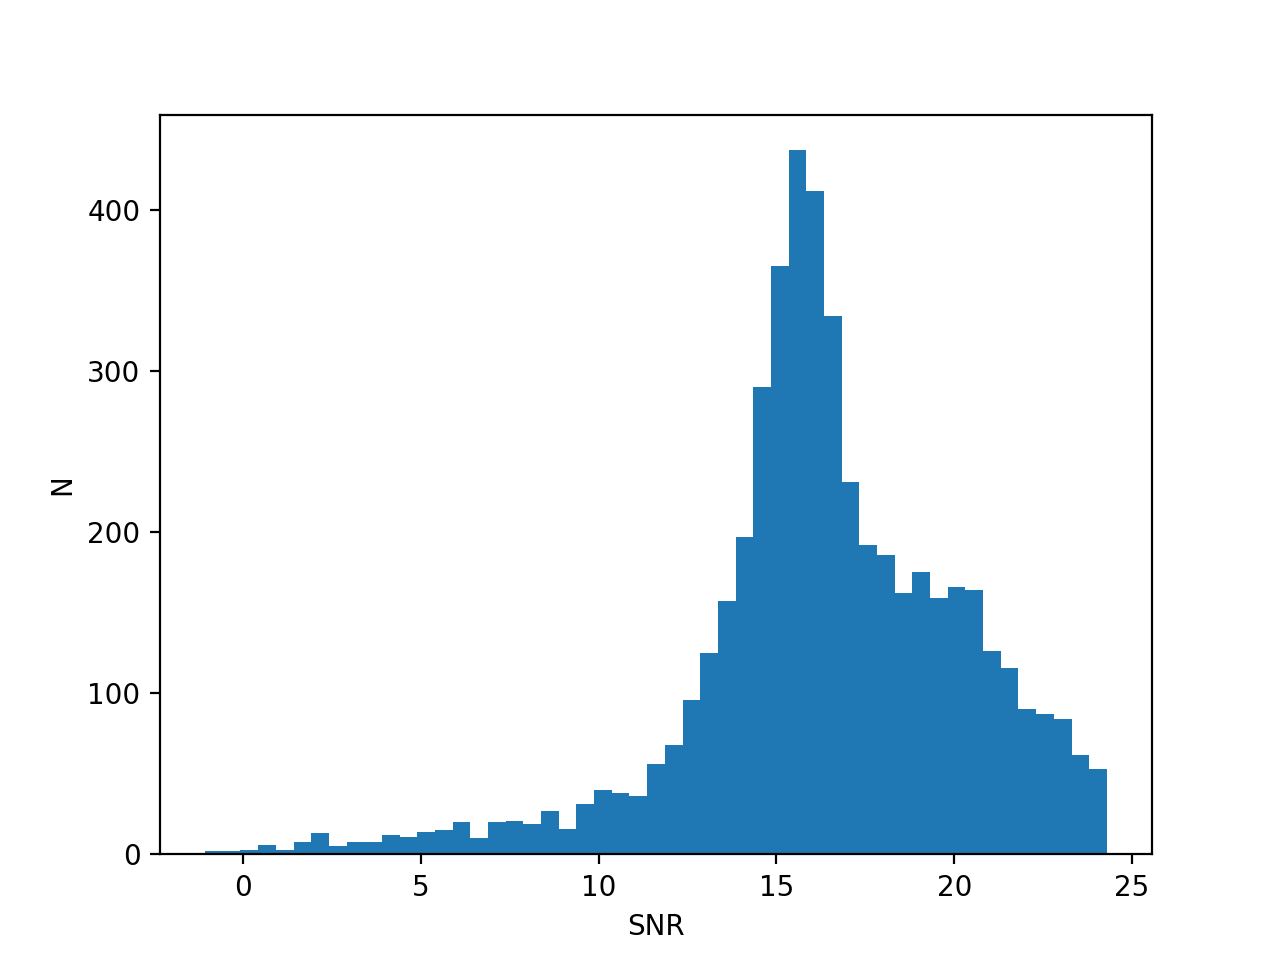
\includegraphics[scale=0.9]{Dataset_SNR}
\caption{Зашумленість набору тренувальних даних} \label{fig:SNR}
\end{center} \end{figure}

На Рис.~\ref{fig:SNR} зображено гістограму, де висота стовбчика ілюструє 
кількість семплів в датасеті з відповідним значенням SNR.

Для перевірки можливостей нейронного радіо вирізняти різні види сигналів 
розглянемо відразу ряд збуджувальних імпульсів:

\begin{equation} \label{eq:type_void}
f_0 = void = 0;
\end{equation}
%
\begin{equation} \label{eq:type_sinc}
f_1 = sinc = \sinc(t-\tau/2);
\end{equation}
%
\begin{equation} \label{eq:type_gauss}
f_2 = gauss = \exp(- (t-\tau/2)^2 );
\end{equation}
%
\begin{equation} \label{eq:type_gauss_perp}
f_3 = gauss\_perp = \partder{}{t} \exp(- (t-\tau/2)^2 );
\end{equation}
%
тоді отриманий набір даних матиме 4 класи, де окремим класом є білий шум. Для
дотримання збалансованості даних в процесі навчання, до раномайзера додамо 
випадковий рівномірно розподілений дискретний параметр, що відповідатиме 
за тип збудження: \textit{void}, \textit{sinc}, \textit{gauss}, 
\textit{gauss\_perp}.

Процес навчання штучної нейронної мережі може проходити як на комп'ютері так і 
на апаратному модулі, за рахунок створення спеціальних програмних драйверів
до апаратної частини \textcolor{red}{[ПОСИЛАННЯ]}. В межах даного дослідження 
достатньо навчання на комп'ютері, як на ресурсах CPU так і на ресурсах GPU.
Для цього набір тренувальних даних необхідно дискритизувати.

Тобто, кожен семпл тренувального набору складатиметься з часової
послідовності, що відповідає прийнятому сигналу та метаданих, що описують 
переданий сигнал: значення енергетичного SNR, тип збудження, 
точка спостереження, ефективна тривалість збудження та інше.

\textcolor{red}{TODO: порівняти методи навчання NLP з DeepUWB}

%%%%%%%%%%%%%%%%%%%%%%%%%%%%%%%%%%%%%%%%%%%%%%%%%%%%%%%%%%%%%%%%%%%%%%%%%%%%%%%
\section{Моделювання детекції сигналу на базі нейронного радіо}

Розглянемо декілька моделей нейронних мереж та визначимо недоліки та переваги
кожної з них. Зоопарк мереж, що розглядається звузимо лише до тих, які 
просто виготовляти. Перші моделі штучних нейронних мереж прямого 
розповсюдження, що були запропоновані - повнозв'язні з одним прихованим шаром.

\textcolor{red}{TODO: плавні активаційні функції через аналогову імплементацію}

\begin{figure}[htbp] \begin{centr}
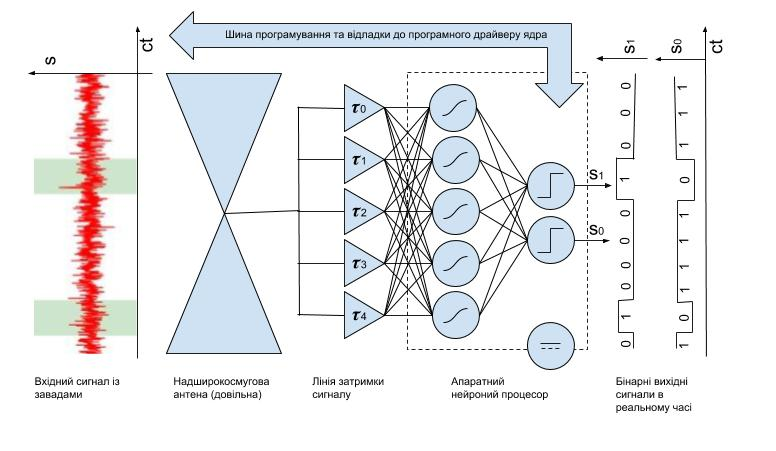
\includegraphics[scale=0.65]{simple_radio}
\caption{Імпульсне радіо на основі багатошарового персептрону} 
\label{fig:mp_radio}
\end{center} \end{figure}

Такі мережі є були популярним засобом розв'язання задач різного типу 
\textcolor{red}{[MNIST]} в основному через досить простий алгоритм навчання.
Для подачі часової послідовності (сигналу) на її вхід обов'язковим стає його 
затримка, що фактично дискредитує вихідний сигнал з антени та втрачає частину 
даних. Такий підхід забезпечує подачу до нейронної мережі деякого 
дискредитованого "вікна" даних та не враховує результат обробки минулого 
вікна при переході до наступного. 

Можна підрахувати, що розмірність вхідного шару визначається частотою 
дискретизації. Для імпульсів переданої антеною типу LIRA з одиничним 
електричним розміром вхідний шар складатиметься не менше ніж з 300 штучних 
нейронів. Так як сигнал може знаходитись в будь-якій частині вікна прихований 
шар повинен містити не меншу кількість нейронів для збереження якісного 
результату в кожен момент часу. З іншого боку, для більшості задач 
електродинаміки важливо знайти, що сигнал взагалі був в якомусь з вікон
що накладаються, тому кількість нейронів в другому шарі можна дещо зменшити.
Останній вихідний шар, що виконує функцію декореру матиме розмірність 
якісної або кількісної характеристики, яку передбачає постанова задачі.
У випадку що розглядається - це тип збудження, який може приймати чотири 
дискретні значення. Таким чином кількість параметрів, що підлягають 
тренуванню - $ 76400 $.

Не дивлячись, на величезну кількість тренувальних параметрів воно проходить 
досить швидко за рахунок малої глибини моделі.

\begin{figure}[htbp] \begin{center}
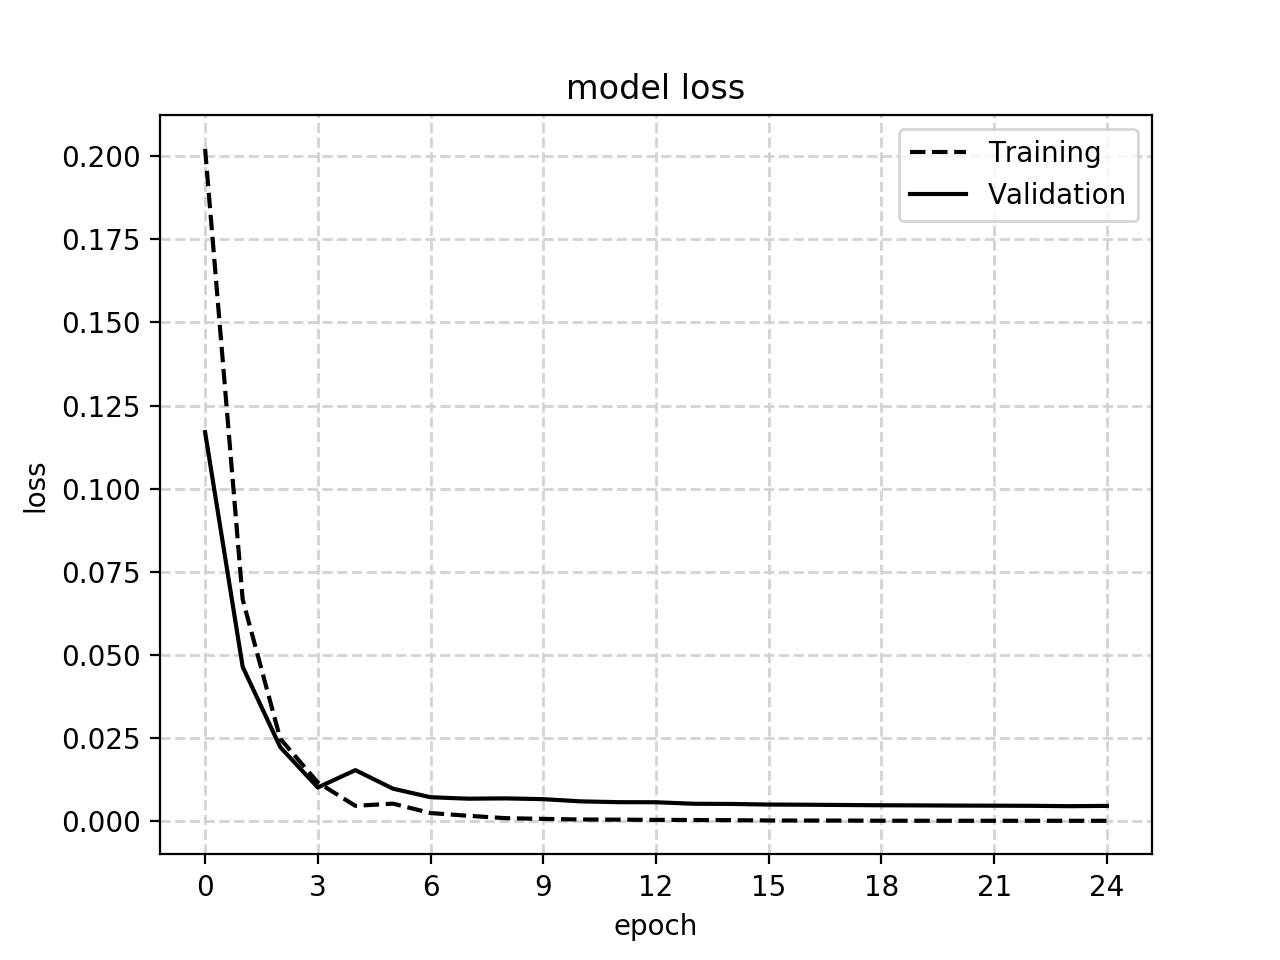
\includegraphics[scale=0.9]{FC_S2L_loss}
\caption{Зміна значення цільової функції повнозв'язної моделі  
в процесі тренування} \label{fig:fcnn_loss}
\end{center} \end{figure}

На Рис.~\ref{fig:fcnn_loss} зображено зміну значень цільової функції в 
процесі тренування порахованої на пренувальних та на тестувальних даних.
Перетин значень цільової функції після третьої епохи є індикатором 
перенавчання моделі. Для тренування використовувалась техніка Dropeout, 
що в купі з перенавчанням є фактором, що вказує на недостатню інформаційну
ємність повнозв'язної моделі для розв'язання поставленої задачі.

Задачею радіоприймача є перетворення в реальному часі сигналу з антени в 
деяку послідовність корисних даних. За класифікацією задач аналізу даних, 
ця задача підходить, як до задач many-to-many, коли кожному елементу 
послідовності відповідає так і до задач many-to-one. Повнозв'язна нейронна
мережа працює саме за схемою many-to-one, коли деякому вікну, що 
спостерігається призначається одна якісна характеристика -
вектор імовірностей присутності сигналів кожного з видів.

Точність роботи алгоритму за метрикою середньої відносної помилки
матиме сенс лише на третій епосі через проблему перенавчання далі, яка 
призводить до втрати точності на реальних даних \textcolor{red}{[ПОСИЛАННЯ]}. 
Таким чином мінімальне значення середньої відносної помилки для штучної 
нейронної мережі пов'язаного типу складе $ 89 \% $.

Серед недоліків застосування описаної архітектури в якості нейронного радіо
можна відмітити велику кількість тренувальних параметрів, що ускладнить 
електронну схему пристрою. Цю проблему можна вирішити використанням 
рекурентних штучних нейронних мереж, які одномоментно приймають на вхід 
одне значення часової послідовності і накопичують інформацію про сигнал 
з плином часу за рахунок зміни свого внутрішнього стану 
\textcolor{red}{[ПОСИЛАННЯ]}.

На відміну від повнозв'язної моделі, рекурентні можуть працювати як за схемою
many-to-one так і за схемою many-to-many, коли в кожен момент часу деякому 
вхідному сигналу співвідноситься якісна або кількісна вихідна характеристика.

У випадку many-to-one вірний прогноз нейронної мережі стосується вікна цвілому, 
а отже точність визначення меж сигналу у часі буде визначена розміром вікна 
спостереження, яке в декілька разів ширше за сигнал. Моделі, що працюють за 
схемою many-to-many позбавлені цього недоліку.

Так як режим роботи нейронної мережі, а тобто many-to-one або many-to-many,
визначається алгоритмом тренування, апаратна реалізація пристрою залишається 
однаковою для many-to-one і many-to-many схем, що зручно для прикладного 
застосування.

Проста архітектура та мала кількість тренувальних параметрів є 
перевагами класичної топології рекурентної штучної нейронної мережі.
Її основним недоліком є нестабільність процесу навчання 
\textcolor{red}{[ПОСИЛАННЯ]} - проблеми exploding gradient і 
vanishing gradient. Саме для вирішення цих проблем були створені архітектури 
GRU \textcolor{red}{[ПОСИЛАННЯ]} та LSTM \cite{imp:Hochreiter1997}.

\begin{figure}[htbp] \begin{center}
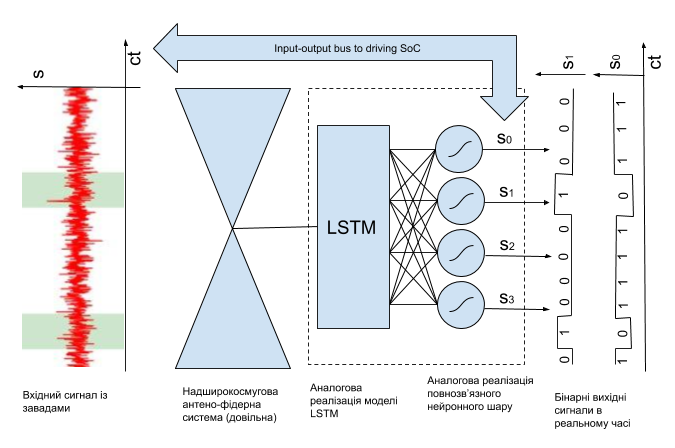
\includegraphics[scale=0.7]{lstm_radio}
\caption{Імпульсне радіо на основі нейронної мережі 
довго-короткотривалої пам'яті} \label{fig:lstm_radio}
\end{center} \end{figure}

На Рис.~\ref{fig:lstm_radio} зображено нейронне радіо з використанням 
рекурентних штучних нейронних мереж. Вихідний шар (decoder) залишився без 
змін - його розмірність визначається практичними потребами. В поточному 
досліді нейрони останнього шару мають сигмоїдальні активаційні функції 
та відповідають імовірностям спостерігати сигнал певного типу. Вхідний 
шар ШНМ є рекурентним, тобто закладається з ланцюжку однакових нейронів.
Описана штучна нейронна мережа має лише 38-116 змінних параметрів в 
залежності від типу рекурентного шару.

Розгладнемо в якості вхідного шару LSTM ланцюжок. Його перевага над 
GRU в контексті нейронного радіо - універсальність: він працює як за схемою
many-to-one так і за схемою many-to-many. Єдиним недоліком LSTM у порівнянні 
з GRU топологією стане більш тривале розповсюдження сигналу крізь такий шар,
що можна нівелювати використовуючи менший техпроцес.

Спершу розглянемо режим роботи many-to-one, щоб порівняти результат з 
повнозвучною нейронною мережею.

\begin{figure}[htbp] \begin{center}
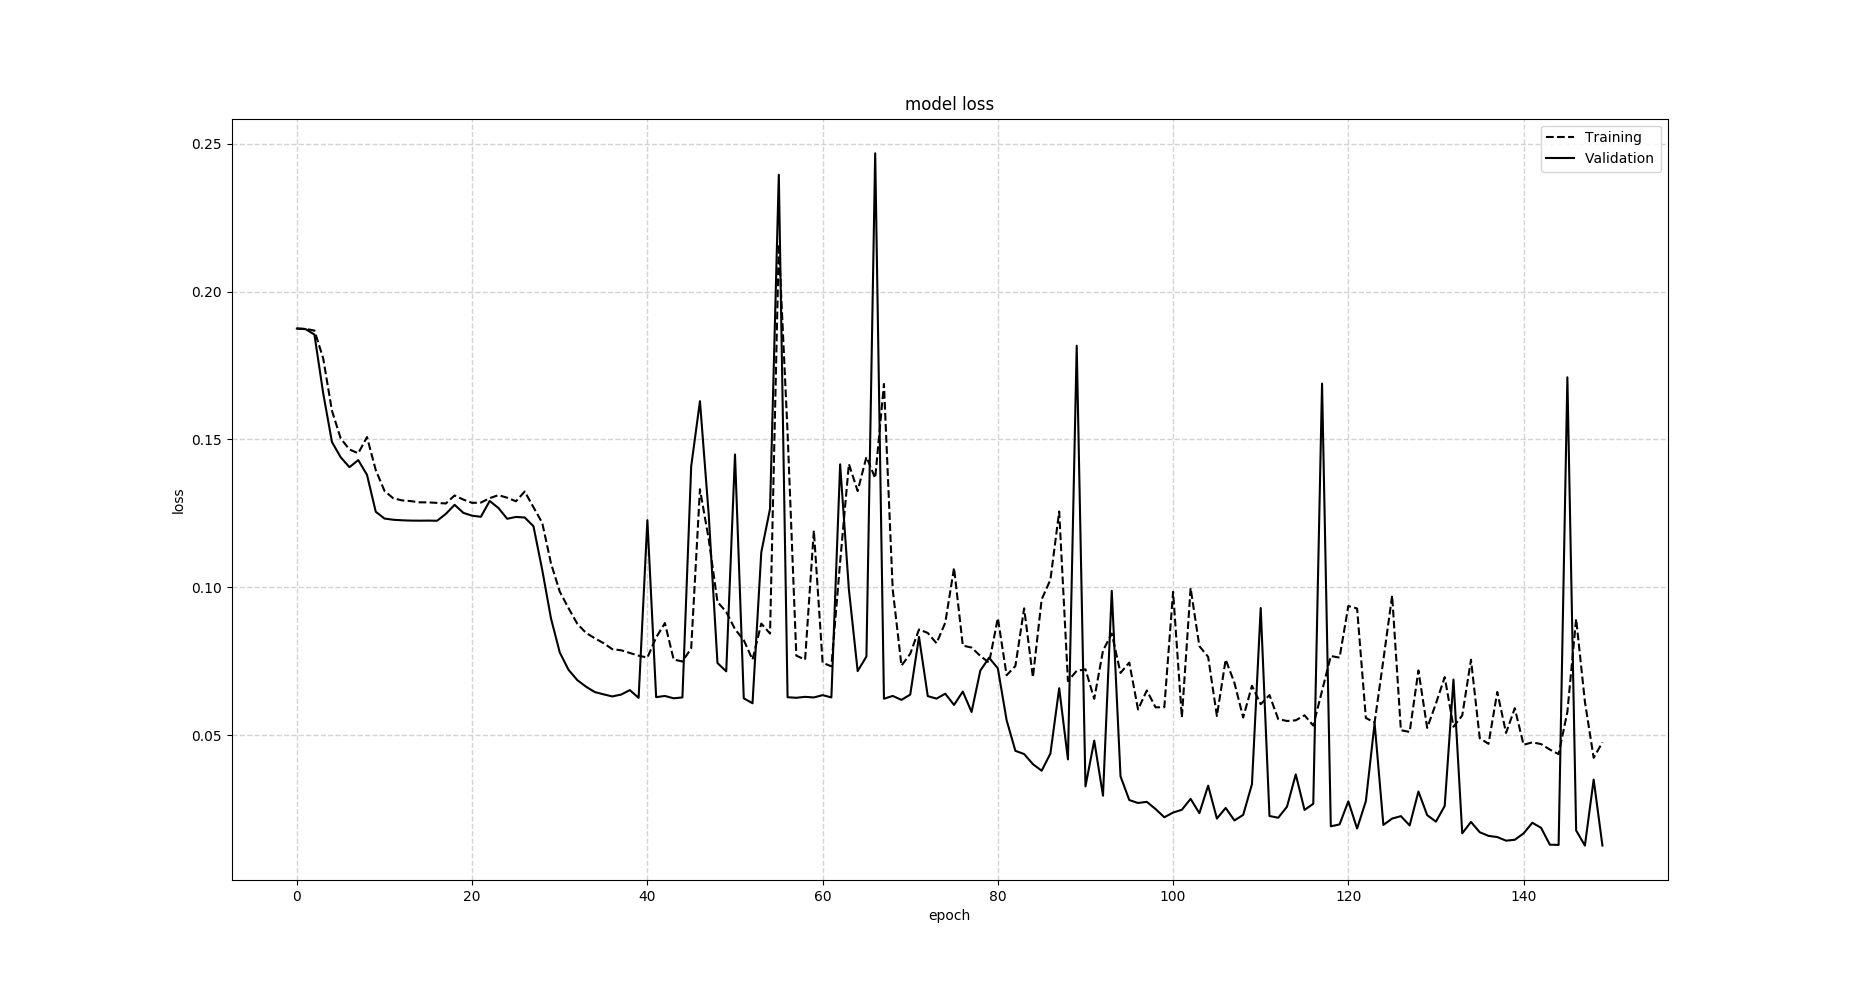
\includegraphics[scale=0.35]{LSTM_S2L_loss}
\caption{Зміна значення цільової функції моделі LSTM 
в процессі тренування} \label{fig:lstm_loss}
\end{center} \end{figure}

На Рис.~\ref{fig:lstm_loss} зображено зміну значень цільової функції в процесі
тренування на тестових та тренувальних даних. Помічаємо, що швидкість навчання 
не рівномірна - спостерігаються "плато" зі сталими значеннями цільової функції,
не приймаючи до уваги випадкових викидів. Подальший аналіз показав, що кожен з 
таких відрізків відповідає за навчання розпізнаванню кожного з типу сигналів, 
що вивчаються. Як можна помітити на малюнку, кожен наступний тип сигналу 
вивчається довше минулого. Порядок вивчання імпульсів теж виявився не 
випадковим: чим більше осциляцій відносно нуля має імпульс тим довше і 
пізніше він вивчається.

Використовуючи рекурентні шари нейронної мережі можна досягти точності в 
$ 99.7\% $, що значно перевищує результати повнозв'язної нейронної мережі 
за рахунок топологічному врахуванню природи електромагнітних хвиль - 
принципу причинності і принципу суперпозиції. Однак, з 
рис.~\ref{fig:lstm_loss} видно, що використання рекурентних нейронних мереж 
помітно сповільнює процес навчання - кількість епох тренування зросла на 
два порядки.

Розглянемо тренування за моделлю many-to-many. Топологія мережі залишається 
як на рис.~\ref{fig:lstm_radio}, а дані для тренування доповнимо анотацією 
для кожного моменту часу замість анотування деякого вікна спостереження.

\begin{figure}[htbp] \begin{center}
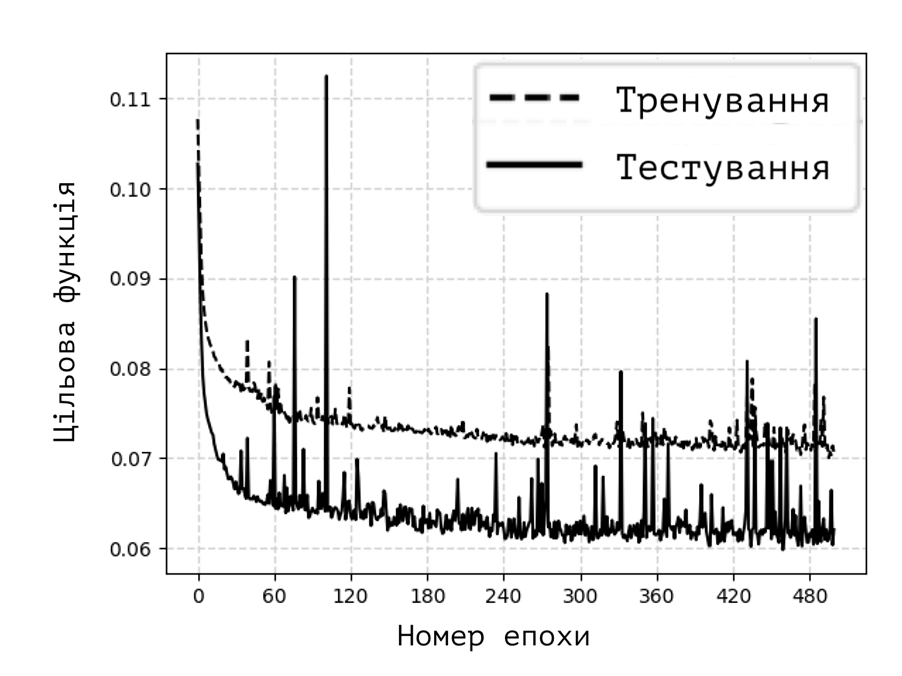
\includegraphics[scale=0.9]{lstm-seq2seq-loss}
\caption{Зміна значення цільової функції моделі LSTM
в процессі тренування} \label{fig:lstm_seq2seq_loss}
\end{center} \end{figure}

На Рис.~\ref{fig:lstm_seq2seq_loss} зображено зміну значень цільової функції
для задачі маркування послідовності (many-to-many). Тут зображено процес 
навчання штучної нейронної мережі на рис.~\ref{fig:lstm_radio} вгадувати 
чи присутній сигнал в певний момент часу, який саме і з якою імовірністю.
При переході від many-to-one до many-to-many тренування сповільнилось. 

\begin{figure}[htbp] \begin{center}
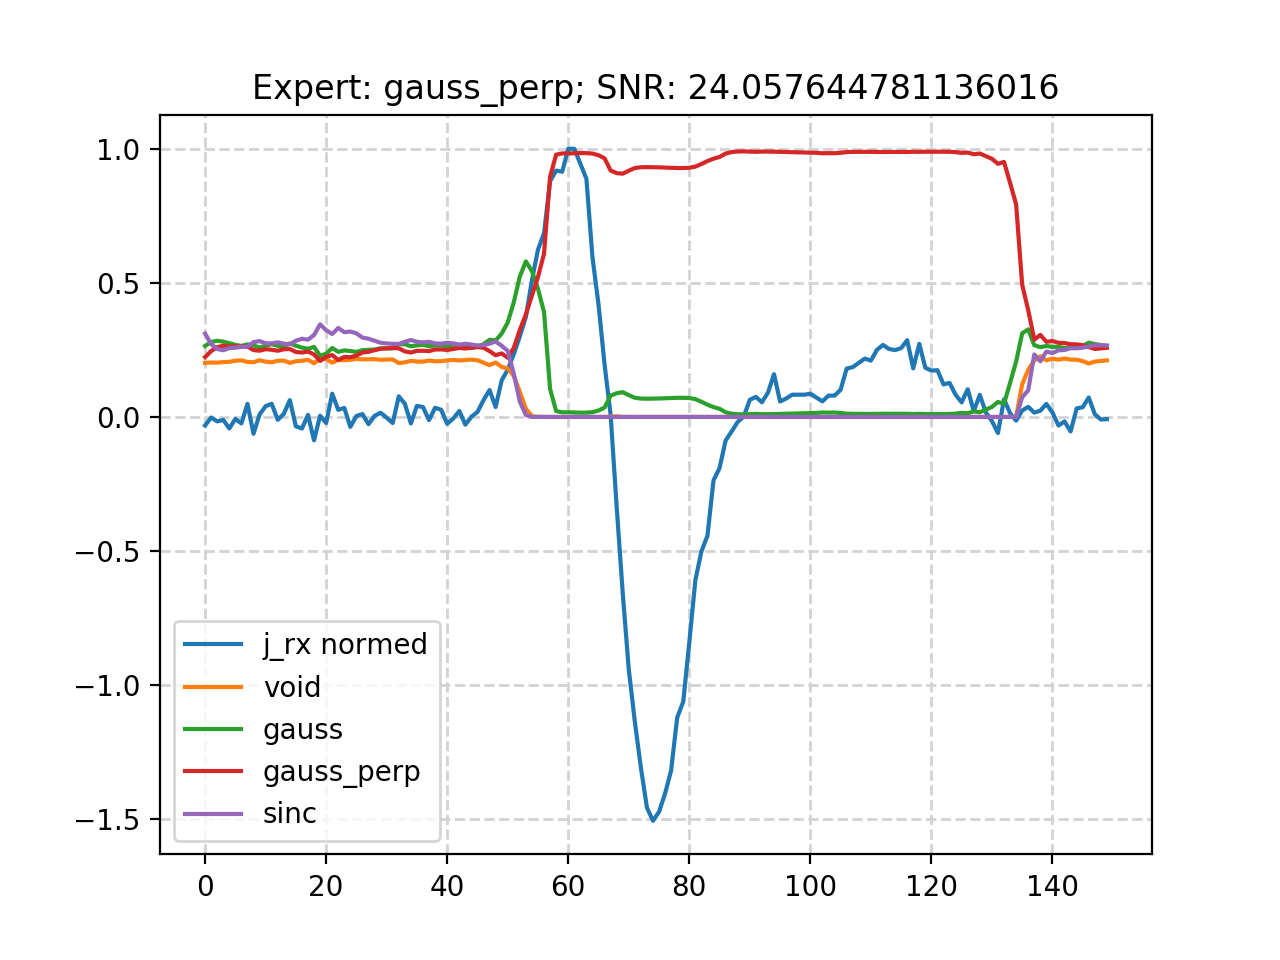
\includegraphics[scale=0.9]{seq2seq_example}
\caption{Приклад правильного аналізу} \label{fig:seq2seq_example}
\end{center} \end{figure}

На Рис.~\ref{fig:lstm_seq2seq_loss} зображено приклад роботи рекурентної 
штучної нейронної мережі для класифікації прийнятого надширокосмугового сигналу 
в кожен момент часу. В представленому зразку даних спостерігається сигнал,
породжений збудженням антени типу LIRA, що має часову залежність у вигляді 
похідної від Гаусіна \eqref{eq:type_gauss_perp} та спостерігається з 
таким відхиленням від осі $ OZ $, що збуджене поле спостерігається, як 
\eqref{eq:type_gauss}. Також на рисунку зображені імовірності приналежності 
сигналу в кожен момент часу до певного збудження чи шуму (відсутності 
збудження).

Для проміжку часу, що передує видимому імпульсу імовірності залишаються 
приблизно рівними та складають близько $ 25 \% $. Тобто при спостеріганні 
білого шуму завчання виходу нейронної мережі, що відповідає на нього 
фактично не правильне. Не дивлячись на це, наявність сигналу можна визначити
аналізуючи всі вихідні значення ШНМ - якщо імовірності наявності сигналів 
кожного з типів (в тому числі і його відсутності) рівні, то спостерігається 
лише шум. Це можна пояснити тим, що нейронна мережа намагається виділити в 
шумі сигнал кожної з вивчених форм, а не знайшовши сигналу повертає 
мінімальний рівноімовірний результат. 

Така систематична методична похибка легко виявляється та нейтралізується 
евристичним аналізом, а також є типовим недоліком в деяких підходах 
розв'язання задач сегментації \textcolor{red}{[ПОСИЛАННЯ]}, яким є задача
маркування послідовності в термінології задач комп'ютерного зору.

На рис.~\ref{fig:lstm_seq2seq_loss} проілюстровано, що навіть у ближній зоні, 
де форма імпульсу може змінюватись на стільки, що стає більше схожою на іншу
нейронне радіо гарантує стійкий режим роботи. З моменту, коли сигнал 
візуально спостерігається, деякий час імовірність відразу за декількома 
ознаками зростає. Далі, мережа визначається з вибором і тримає його весь
час тривалості сигналу. Стійка детекція сигналу за значенням трешхолду 
$ 0.707 $ займає близько $ 70\% $ тривалості сигналу.

Точність роботи мережі на валідаційному датасеті впала до $ 98.9\% $,
що є закономірним при підвищенні точності визначення тривалості сигналу.

\begin{figure}[htbp] \begin{center}
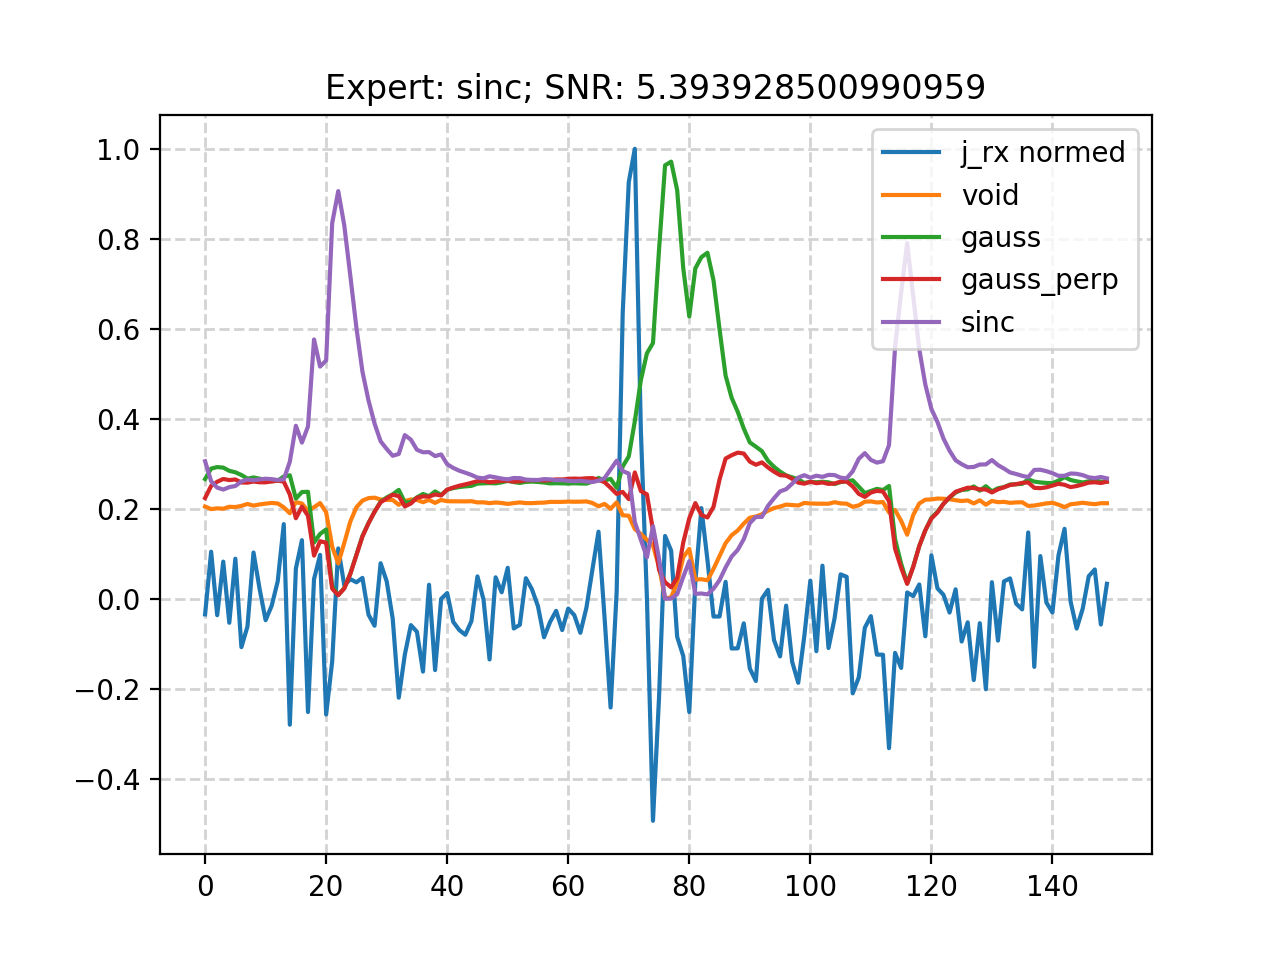
\includegraphics[scale=0.9]{lstm_seq2seq_bad}
\caption{Приклад не правильного аналізу} \label{fig:lstm_seq2seq_bad}
\end{center} \end{figure}

На рис.~\ref{fig:lstm_seq2seq_bad} зображено приклад неправильного
розпізнавання сигналу. Зразок містить сигнал, породжений збудженням антени 
типу LIRA, що має часову залежність у вигляді sampling function 
\eqref{eq:type_sinc}. Рекурентна штучна нейронна мережа надала нестійку
детекцію трьох сигналів в хронологічній послідовності: \textit{sinc}, 
\textit{gauss}, \textit{sinc}. Детекція першого сигналу викликана 
одномоментною схожістю сигналу на \textit{sinc}, що викликало ланцюжкову 
реакцію для подальших помилкових детекції сигналів: мережа гадає, що 
помилково детектований сигнал накладається на реальний сигнал і робить 
невірне передбачення класу його приналежності.

\textcolor{red}{TODO: HMM для захищеного радіо-вимикача }

%%%%%%%%%%%%%%%%%%%%%%%%%%%%%%%%%%%%%%%%%%%%%%%%%%%%%%%%%%%%%%%%%%%%%%%%%%%%%%%
\section{Оцінка стійкості апаратних нейронних мереж до внутрішніх шумів}

%%%%%%%%%%%%%%%%%%%%%%%%%%%%%%%%%%%%%%%%%%%%%%%%%%%%%%%%%%%%%%%%%%%%%%%%%%%%%%%
\section{Універсальна топологія нейронного радіо та її застосування}

\textcolor{red}{TODO: триваліть прехідної функції мосфета }

\textcolor{red}{TODO: какое ограничение по длительности и амплитуде импульса}

\textcolor{red}{ (fully connected) calculation graph -> (LSTM) принцип 
причинності закладений в архітектуру -> (attention) кажемо моделі де 
найважливіщі з точки зору інформації місця, що спостервгаються в сигналі 
(важливо для більшості задач сучасної радіофізики) bidirectional lstm -> 
можна використати знання про сигнал, щоб якісніше оцінити модель шуму в 
реальному часі}

Перед усім, досвід машинного навчання в сфері обробки часових послідовностей 
стверджує що, доцільніше аналізувати не сигнал а його числові характеристики. 
Самі характеристики можуть бути різними та визначатись довільно. 
Головна вимога до набору параметрів, які описують сигнал - вони повинні 
однозначно вирізняти всі сигнали, що можуть бути прийняті антенною 
системою. В якості таких параметрів пропонується використовувати апаратне 
MFCC перетворення або деяку систему зі штучних нейронів, яка визначить набір 
параметрів автоматично. Не рекомендується використовувати різні евристичні та 
статистичні числові характеристики в якості параметрів сигналу.

Перед перетворенням сигналу на набір властивостей може використовуватись 
нейронна мережа зниження рівня шумів denoising autoencoder (NDA), 
яка покращить співвідношення сигналу до шуму. Для покращення роботи 
NDA можна накопичити минулі вікна спостереження, що додасть 
інформації про шум.

\textcolor{red}{Зазвичай, надширокосмугова імпульсна радіолокація виконується 
через вимірювання часу надходження відбитого випромінювання. Використання 
нейроної мережі дозволить підвищити точність такого вимірювання через 
визначення не тільки часу, а і азимутального кута прийому. Для цього навчимо 
нейронну мережу розпізнавати напрямок до цілі за формою імпульсу, яка сильно 
змінюється у ближній зоні.}

\textcolor{red}{TODO: Задача радіовимірювань при нелінійних спотворенях сигналу}

\textcolor{red}{TODO: генерація сигналу для передачі декодером мережі для 
розв'язання задач адаптивних антен, або для випромінювання сигналу-відповіді 
на вхідний запит по радіоаналу}

\begin{equation}
C = \frac{1}{N_{smp}} \frac{\log_2 \left( 1 + SNR \right)}{1/B + \tau_{RMS}} 
\end{equation}

\begin{figure}[htbp] \begin{center}
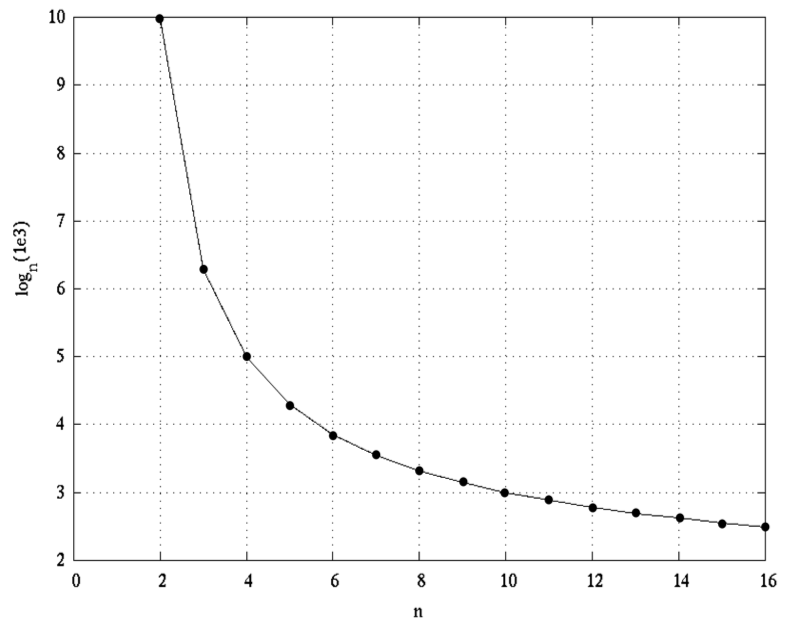
\includegraphics[scale=0.7]{channel_capacity}
\caption{Інформаційна емність імпульсного випромінювання} \label{fig:info_cap}
\end{center} \end{figure}

\textcolor{red}{TODO: При виготовлені складних антен, наприклад лінзевих, часто
виникають виробничі дефекти. Методика переносу навчання дозволяє адаптувати 
гарно натреновану на теоретичних даних модель під такі реальні умові. Також
це дозволяє адаприувати систему під унікальні завади, які можна зустріти,
наприклад, в іоносфері }

\textcolor{red}{TODO: Провести аналогію до image classification transfer 
learing}
